\documentclass[12pt]{article}
\usepackage[margin=1in]{geometry}
\usepackage{booktabs}
\usepackage{graphicx}
\usepackage{float}
\usepackage{amsmath}
\usepackage[colorlinks=true,linkcolor=black,citecolor=black,urlcolor=blue]{hyperref}
\usepackage{setspace}
\usepackage[T1]{fontenc}
\usepackage{lmodern}
\usepackage{natbib}

\onehalfspacing
\graphicspath{{output/}}
\newcommand{\sym}[1]{\ensuremath{^{#1}}}

\title{AI-Based Interventions and Perceived Bias in News Coverage of China: Primary Analysis}
\author{}
\date{April 2026}

\begin{document}
\maketitle

\begin{abstract}
\noindent We study the effects of AI-based interventions on perceptions of bias in news coverage of China using a pre-registered online experiment ($N=1{,}017$; US, UK, and Canada). Participants read a news article and were randomly assigned to one of three treatments varying in interactivity: an interactive AI chatbot, a tailored AI-generated comment, or a generic static message. Taking the static message as the baseline, the chatbot significantly increases perceived bias against China by approximately 8.5 points on a 0--100 scale ($p<0.001$). The comment produces an intermediate effect ($+5.3$ points, $p=0.008$). No significant treatment differences are found for perceived trustworthiness or sharing intentions; both the chatbot and comment increase perceived one-sidedness. Treatment effects are consistent across all three countries. Exploratory analysis suggests that the verification motive---participants' desire to verify the article further---is the information-processing channel most strongly associated with bias perception change, particularly in the interactive treatments.
\end{abstract}

%============================================================
\section{Experimental Design}
%============================================================

\subsection{Overview}

The experiment studies how AI-generated interventions of varying interactivity affect participants' perceptions of a news article about China. All participants read the same article (``China's Long-Promised Consumer Boom...'') and were randomly assigned to one of three treatment arms:

\begin{itemize}
    \item \textbf{Static} ($n=294$, 28.9\%): A generic static message. This is the baseline condition.
    \item \textbf{Comment} ($n=331$, 32.5\%): A single, tailored AI-generated comment personalized to the participant's stated opinion.
    \item \textbf{Chatbot} ($n=392$, 38.5\%): Interactive AI chatbot conversation with up to 3 rounds of dialogue.
\end{itemize}

\subsection{Outcomes}

Four outcome measures were elicited both before and after treatment on a 0--100 continuous scale:
\begin{enumerate}
    \item \textbf{Primary outcome}: Perceived bias against China.
    \item \textbf{Secondary outcomes}: Perceived trustworthiness, perceived one-sidedness, and sharing likelihood.
\end{enumerate}
The estimand of interest is the change score (post $-$ pre) for each measure.

\subsection{Estimands}

The \textit{primary estimand} is the intent-to-treat (ITT) effect of the Chatbot versus the Static condition on the change in perceived bias against China, controlling for pre-treatment bias. Secondary estimands include the Comment versus Static contrast and all contrasts on the three secondary outcomes.

\subsection{Sample}

Table~\ref{tab:flow} reports the participant flow. The sample comprises participants from three English-speaking countries recruited via Prolific ($N=1{,}017$). No observations are excluded. All participants passed the attention check.

\begin{table}[H]
\centering
\caption{Participant Flow}
\label{tab:flow}
\begin{tabular}{lcccc}
\toprule
 & Static & Comment & Chatbot & Total \\
\midrule
US     & 87  & 106 & 140 & 333 \\
UK     & 97  & 109 & 131 & 337 \\
Canada & 110 & 116 & 121 & 347 \\
\midrule
Total  & 294 & 331 & 392 & 1,017 \\
\bottomrule
\end{tabular}
\par\vspace{4pt}
\begin{minipage}{\textwidth}
\footnotesize \textit{Notes:} No exclusions applied. All participants passed the recall-based attention check.
\end{minipage}
\end{table}

%============================================================
\section{Summary Statistics and Balance}
%============================================================

Table~\ref{tab:summary} reports summary statistics by treatment group. Panel A presents demographic characteristics with $p$-values from OLS regressions of each covariate on treatment indicators. Most covariates are well-balanced. Trust in AI ($p=0.001$) and income ($p=0.041$) show some imbalance; both are controlled for in the full specification with no meaningful change in estimates. Panel B reports the race distribution. Pre-treatment outcome levels are well-balanced across arms (all $p>0.50$; not shown).

\begin{table}[htbp]
\centering
\caption{Summary Statistics}
\label{tab:summary}
\small
\begin{tabular}{l*{4}{c}c}
\toprule
 & Static & Comment & Chatbot & Total & $p$-value \\
 & (1) & (2) & (3) & (4) & (5) \\
\midrule
\addlinespace
\multicolumn{6}{l}{\textit{Panel A: Demographics}} \\
\addlinespace
Age & 47.47 & 45.87 & 45.81 & 46.28 & 0.531 \\
    & (17.04) & (16.28) & (15.96) & (16.36) & \\
\addlinespace
Female (\%) &  0.48 &  0.56 &  0.51 &  0.52 & 0.217 \\
\addlinespace
Income (1--10) &  5.06 &  5.49 &  5.53 &  5.39 & 0.012 \\
    & ( 1.82) & ( 1.73) & ( 1.62) & ( 1.72) & \\
\addlinespace
Education &  3.01 &  2.98 &  3.09 &  3.03 & 0.509 \\
    & ( 1.24) & ( 1.01) & ( 1.16) & ( 1.14) & \\
\addlinespace
Pol.\ orientation (1--7) &  3.90 &  3.80 &  3.89 &  3.86 & 0.752 \\
    & ( 1.51) & ( 1.62) & ( 1.60) & ( 1.58) & \\
\addlinespace
Trust in AI (1--7) &  4.09 &  4.30 &  4.47 &  4.31 & 0.016 \\
    & ( 1.43) & ( 1.51) & ( 1.37) & ( 1.44) & \\
\addlinespace
Favorable to China (1--5) &  3.08 &  3.08 &  3.16 &  3.11 & 0.534 \\
    & ( 0.83) & ( 1.00) & ( 0.87) & ( 0.90) & \\
\addlinespace
\multicolumn{6}{l}{\textit{Panel B: Race/Ethnicity (\%)}} \\
\addlinespace
White    & 77.2 & 77.2 & 74.9 & 76.3 & \\
Black    &  7.1 &  5.6 & 11.8 &  8.5 & \\
Hispanic &  5.4 &  4.2 &  3.7 &  4.3 & \\
Asian    &  7.1 &  7.9 &  5.9 &  6.9 & \\
Mixed/Other &  3.3 &  5.1 &  3.7 &  4.0 & \\
\midrule
Observations & 184 & 215 & 271 & 670 & \\
\bottomrule
\end{tabular}
\par\vspace{4pt}
\begin{minipage}{\textwidth}
\footnotesize \textit{Notes:} Standard deviations in parentheses. Column (5) reports $p$-values from OLS regressions of each covariate on treatment indicators with robust standard errors. Race distribution tested with Pearson $\chi^2$ ($p = 0.501$).
\end{minipage}
\end{table}


%============================================================
\section{Treatment Effects}
%============================================================

\subsection{Primary Result: Perceived Bias Against China}

Figure~\ref{fig:panel} displays mean within-arm change scores (post $-$ pre) with 95\% confidence intervals. The bottom-left panel shows the key pattern: the Chatbot arm exhibits a large increase in perceived bias against China, the Comment arm an intermediate increase, and the Static arm essentially no change. All three arms show comparable declines in perceived trustworthiness (top-left).

\begin{figure}[H]
\centering
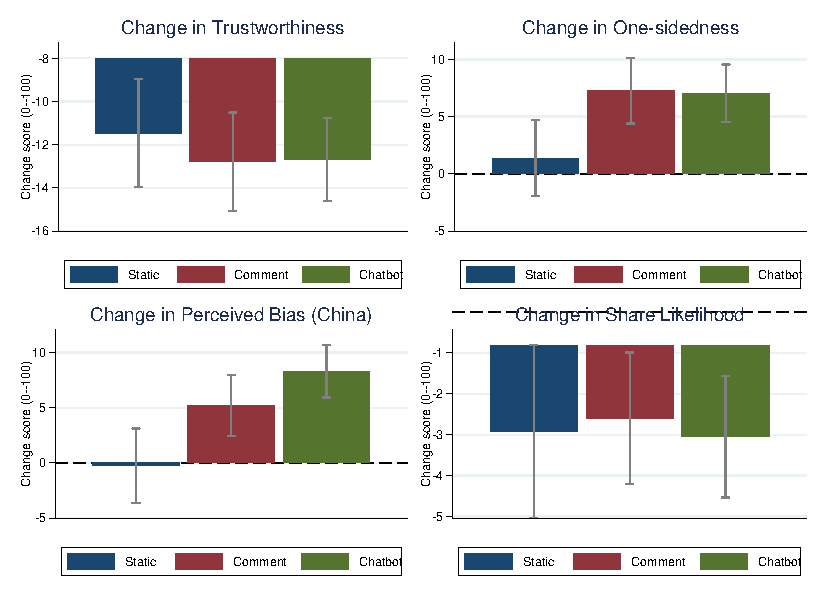
\includegraphics[width=\textwidth]{fig1_panel.pdf}
\caption{Changes in News Perceptions by Treatment (with 95\% CIs)}
\label{fig:panel}
\end{figure}

Table~\ref{tab:bias} presents the primary estimand---the between-arm treatment effect relative to Static---across three specifications. The Chatbot effect is large and robust across all specifications ($p<0.001$). With the addition of Canada to the sample, the Comment effect is now also statistically significant in the preferred specification (column 2: $\beta = 5.27$, $p = 0.008$).

\begin{table}[htbp]
\centering
\caption{Treatment Effects on Perceived Bias Against China}
\label{tab:bias}
\begin{tabular}{l*{3}{c}}
\toprule
 & \multicolumn{3}{c}{Change in Perceived Bias (0--100)} \\
                    &\multicolumn{1}{c}{(1)}&\multicolumn{1}{c}{(2)}&\multicolumn{1}{c}{(3)}\\
                    &\multicolumn{1}{c}{(1)}&\multicolumn{1}{c}{(2)}&\multicolumn{1}{c}{(3)}\\
\midrule
Chatbot             &       9.366\sym{***}&       8.894\sym{***}&       8.605\sym{***}\\
                    &     (2.575)         &     (2.332)         &     (2.321)         \\
\addlinespace
Comment             &       4.051         &       3.602         &       3.259         \\
                    &     (2.790)         &     (2.500)         &     (2.512)         \\
\addlinespace
Pre-treatment bias  &                     &      -0.428\sym{***}&      -0.431\sym{***}\\
                    &                     &     (0.040)         &     (0.041)         \\
\addlinespace
Age                 &                     &                     &      -0.082         \\
                    &                     &                     &     (0.057)         \\
\addlinespace
Female              &                     &                     &       2.662         \\
                    &                     &                     &     (1.818)         \\
\addlinespace
Education           &                     &                     &       0.824         \\
                    &                     &                     &     (0.899)         \\
\addlinespace
Income              &                     &                     &      -0.346         \\
                    &                     &                     &     (0.571)         \\
\addlinespace
Pol.\ orientation   &                     &                     &      -0.898         \\
                    &                     &                     &     (0.641)         \\
\addlinespace
Trust in AI         &                     &                     &       0.179         \\
                    &                     &                     &     (0.663)         \\
\addlinespace
Favorable to China  &                     &                     &       0.597         \\
                    &                     &                     &     (1.079)         \\
\addlinespace
UK                  &                     &                     &      -0.978         \\
                    &                     &                     &     (1.833)         \\
\midrule
Observations        &         670         &         670         &         670         \\
$R^2$               &       0.022         &       0.201         &       0.212         \\
\bottomrule
\end{tabular}
\par\vspace{4pt}
\begin{minipage}{\textwidth}
\footnotesize \textit{Notes:} OLS estimates. The dependent variable is the change in perceived bias against China (post minus pre) on a 0--100 scale. The omitted baseline is the Static treatment. Robust standard errors in parentheses. Column (1) is unadjusted; column (2) controls for pre-treatment bias; column (3) adds demographic controls and country fixed effect. \sym{*}~$p<0.10$, \sym{**}~$p<0.05$, \sym{***}~$p<0.01$.
\end{minipage}
\end{table}


\subsection{Secondary Outcomes}

Table~\ref{tab:all} reports effects on all four outcomes using the preferred specification (OLS with pre-treatment control). Both Chatbot and Comment significantly increase perceived one-sidedness relative to Static (column 2). Neither treatment significantly affects trustworthiness or sharing intentions.

\begin{table}[htbp]
\centering
\caption{Treatment Effects on All Outcomes}
\label{tab:all}
\begin{tabular}{l*{4}{c}}
\toprule
 & \multicolumn{4}{c}{Change Score (Post $-$ Pre)} \\
\cmidrule(lr){2-5}
                    &\multicolumn{1}{c}{(1)}&\multicolumn{1}{c}{(2)}&\multicolumn{1}{c}{(3)}&\multicolumn{1}{c}{(4)}\\
                    &\multicolumn{1}{c}{Trust}&\multicolumn{1}{c}{One-sided}&\multicolumn{1}{c}{Bias}&\multicolumn{1}{c}{Share}\\
\midrule
Chatbot             &      -2.236         &       3.700\sym{*}  &       8.894\sym{***}&       0.163         \\
                    &     (1.758)         &     (2.185)         &     (2.332)         &     (1.499)         \\
\addlinespace
Comment             &      -1.559         &       1.884         &       3.602         &      -0.036         \\
                    &     (1.909)         &     (2.287)         &     (2.500)         &     (1.591)         \\
\midrule
Observations        &         670         &         670         &         670         &         670         \\
$R^2$               &       0.187         &       0.317         &       0.201         &       0.164         \\
\bottomrule
\end{tabular}
\par\vspace{4pt}
\begin{minipage}{\textwidth}
\footnotesize \textit{Notes:} OLS estimates. Each column reports a separate regression of the change score on treatment indicators and the pre-treatment level of the outcome. The omitted baseline is the Static treatment. Robust standard errors in parentheses. The primary outcome is perceived bias against China (column 3). Columns 1, 2, and 4 report secondary outcomes. \sym{*}~$p<0.10$, \sym{**}~$p<0.05$, \sym{***}~$p<0.01$.
\end{minipage}
\end{table}


Figure~\ref{fig:coefplot} visualizes the treatment effects across all outcomes.

\begin{figure}[H]
\centering
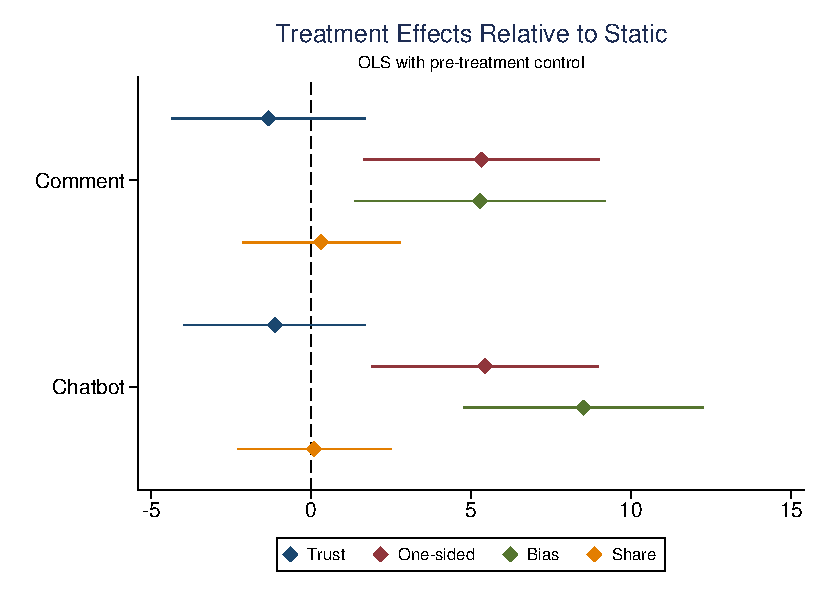
\includegraphics[width=0.85\textwidth]{fig2_coefplot.pdf}
\caption{Treatment Effects Relative to Static}
\label{fig:coefplot}
\end{figure}

\subsection{Robustness: Permutation Tests}

We verify the main results using Fisher-Pitman permutation tests (200,000 Monte Carlo simulations). Table~\ref{tab:perm} reports two-tailed $p$-values.

\begin{table}[H]
\centering
\caption{Pairwise Permutation Tests ($p$-values, Two-Tailed)}
\label{tab:perm}
\begin{tabular}{lccc}
\toprule
Outcome & Chatbot vs.\ Static & Comment vs.\ Static & Chatbot vs.\ Comment \\
\midrule
Bias (primary)  & $<$\textbf{0.001} & \textbf{0.013} & 0.098 \\
Trust            & 0.445 & 0.443 & 0.945 \\
One-sidedness    & \textbf{0.007} & \textbf{0.008} & 0.917 \\
Sharing          & 0.923 & 0.809 & 0.691 \\
\bottomrule
\end{tabular}
\par\vspace{4pt}
\begin{minipage}{\textwidth}
\footnotesize \textit{Notes:} Each cell reports a two-tailed $p$-value from a Fisher-Pitman permutation test (200,000 Monte Carlo simulations) comparing the mean change score between two treatment groups. Bold indicates $p < 0.05$.
\end{minipage}
\end{table}

The primary result---Chatbot significantly increases perceived bias relative to Static---is confirmed nonparametrically ($p<0.001$). The Comment vs.\ Static contrast is also significant ($p=0.013$). Both Chatbot and Comment significantly increase perceived one-sidedness ($p<0.01$).

\subsection{Multiple Hypothesis Testing Corrections}

We address multiplicity along two dimensions. First, we apply Bonferroni-Holm across the three pairwise treatment comparisons on the primary outcome (Panel A of Table~\ref{tab:mht}). Second, we apply the Romano-Wolf stepdown procedure (Romano \& Wolf, 2005) across the four-outcome family for each treatment contrast (Panel B), using 5,000 bootstrap replications.

\begin{table}[H]
\centering
\caption{Multiple Hypothesis Testing Corrections}
\label{tab:mht}
\begin{tabular}{lccc}
\toprule
 & Unadjusted & Bonferroni-Holm & \\
\multicolumn{4}{l}{\textit{Panel A: Three pairwise comparisons on perceived bias}} \\
\midrule
Chatbot vs.\ Static  & $<$0.001 & $<$0.001 & \\
Comment vs.\ Static  & 0.008  & 0.016  & \\
Chatbot vs.\ Comment & 0.056  & 0.056  & \\
\addlinespace
 & Unadjusted & Romano-Wolf & \\
\multicolumn{4}{l}{\textit{Panel B: Four outcomes (Romano-Wolf stepdown)}} \\
\midrule
\multicolumn{4}{l}{\textit{Chatbot vs.\ Static}} \\
\quad Bias            & $<$0.001 & 0.0002 & \\
\quad One-sidedness   & 0.002  & 0.007  & \\
\quad Trust           & 0.420  & 0.637  & \\
\quad Sharing         & 0.932  & 0.931  & \\
\addlinespace
\multicolumn{4}{l}{\textit{Comment vs.\ Static}} \\
\quad Bias            & 0.007  & 0.018  & \\
\quad One-sidedness   & 0.005  & 0.017  & \\
\quad Trust           & 0.412  & 0.642  & \\
\quad Sharing         & 0.790  & 0.796  & \\
\bottomrule
\end{tabular}
\par\vspace{4pt}
\begin{minipage}{\textwidth}
\footnotesize \textit{Notes:} Panel A applies the Holm (1979) step-down procedure across three pairwise comparisons on the primary outcome (perceived bias). Panel B applies the Romano-Wolf (2005) stepdown procedure across four outcomes for each treatment contrast, with 5,000 bootstrap replications and robust standard errors. All regressions control for the pre-treatment level of the outcome.
\end{minipage}
\end{table}

Both the Chatbot and Comment effects on perceived bias survive all corrections. In Panel A, Chatbot vs.\ Static and Comment vs.\ Static are significant after Bonferroni-Holm ($p<0.001$ and $p=0.016$). In Panel B, the Romano-Wolf adjusted $p$-values confirm that the bias result is not an artifact of testing multiple outcomes: the adjusted $p$-values are 0.0002 (Chatbot) and 0.018 (Comment). The one-sidedness result also survives Romano-Wolf correction for both contrasts ($p \leq 0.017$).

Figure~\ref{fig:box} shows the full distribution of change scores by treatment.

\begin{figure}[H]
\centering
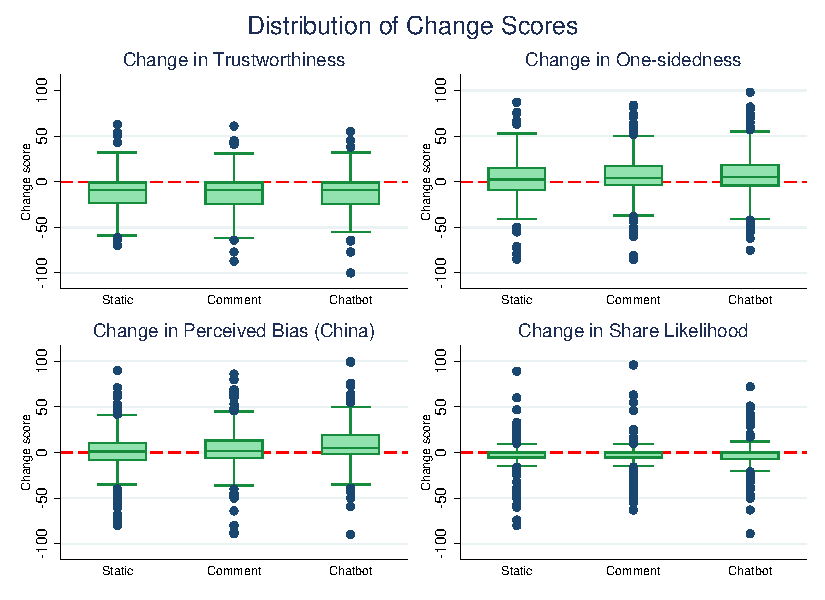
\includegraphics[width=\textwidth]{fig3_boxplots.pdf}
\caption{Distribution of Change Scores by Treatment}
\label{fig:box}
\end{figure}

%============================================================
\section{Country Heterogeneity}
%============================================================

Table~\ref{tab:nation} reports treatment effects on the primary outcome interacted with country indicators (US is the baseline). None of the interaction terms are statistically significant, indicating that the treatment effects are consistent across the US, UK, and Canada. The point estimate for the Comment $\times$ Canada interaction is positive ($+6.98$) but not significant at conventional levels.

\begin{table}[htbp]
\centering
\caption{Treatment Effects by Country}
\label{tab:nation}
\begin{tabular}{lc}
\toprule
                    &\multicolumn{1}{c}{(1)}\\
                    &\multicolumn{1}{c}{Change in Perceived Bias}\\
\midrule
Chatbot             &       8.721\sym{***}\\
                    &     (3.343)         \\
\addlinespace
Comment             &       1.466         \\
                    &     (3.603)         \\
\addlinespace
UK                  &      -2.251         \\
                    &     (3.890)         \\
\addlinespace
Chatbot $\times$ UK &       0.160         \\
                    &     (4.699)         \\
\addlinespace
Comment $\times$ UK &       4.128         \\
                    &     (5.016)         \\
\midrule
Observations        &         670         \\
$R^2$               &       0.202         \\
\bottomrule
\end{tabular}
\par\vspace{4pt}
\begin{minipage}{\textwidth}
\footnotesize \textit{Notes:} OLS estimates. Dependent variable: change in perceived bias against China (0--100). Controls for pre-treatment bias. Baseline: Static treatment in the US. Robust standard errors in parentheses. \sym{*}~$p<0.10$, \sym{**}~$p<0.05$, \sym{***}~$p<0.01$.
\end{minipage}
\end{table}


%============================================================
\section{Exploratory Analysis: Information Processing}
%============================================================

We examine whether three post-treatment information-processing measures predict perception changes differently across treatment arms. The three measures, each on a 1--7 Likert scale, are: (i) \textit{fairness evaluation} (``helped me evaluate whether the article was fair''), (ii) \textit{information novelty} (``the information provided is new to me''), and (iii) \textit{verification motive} (``made me want to verify the article further''). Because these variables are measured after treatment, the results should be interpreted as exploratory within-treatment associations, not as causal mediation.

Table~\ref{tab:withinbias} reports OLS regressions of the change in perceived bias on the three information-processing measures, estimated separately within each treatment arm. The verification motive is positively associated with increased perceived bias in all three arms, but the association is strongest and most precisely estimated in the Comment and Chatbot arms. Information novelty shows no significant association in any arm.

\begin{table}[htbp]
\centering
\caption{Information Processing and Bias Perception Change by Treatment}
\label{tab:withinbias}
\begin{tabular}{l*{3}{c}}
\toprule
 & \multicolumn{3}{c}{Change in Perceived Bias (0--100)} \\
\cmidrule(lr){2-4}
                    &\multicolumn{1}{c}{(1)}&\multicolumn{1}{c}{(2)}&\multicolumn{1}{c}{(3)}\\
                    &\multicolumn{1}{c}{Static}&\multicolumn{1}{c}{Comment}&\multicolumn{1}{c}{Chatbot}\\
\midrule
Fairness evaluation &       2.509\sym{*}  &       0.796         &       1.590         \\
                    &     (1.300)         &     (1.153)         &     (1.103)         \\
\addlinespace
Information novelty &      -0.476         &      -0.686         &      -0.731         \\
                    &     (1.146)         &     (0.837)         &     (0.851)         \\
\addlinespace
Verification motive &       1.252         &       3.313\sym{***}&       2.189\sym{***}\\
                    &     (1.291)         &     (1.053)         &     (0.743)         \\
\midrule
Observations        &         294         &         331         &         392         \\
$R^2$               &       0.215         &       0.254         &       0.205         \\
\bottomrule
\end{tabular}
\par\vspace{4pt}
\begin{minipage}{\textwidth}
\footnotesize \textit{Notes:} OLS estimates within each treatment arm. Dependent variable: change in perceived bias against China (0--100). All regressions control for pre-treatment bias. All information-processing measures are on a 1--7 Likert scale. Robust standard errors in parentheses. \sym{*}~$p<0.10$, \sym{**}~$p<0.05$, \sym{***}~$p<0.01$.
\end{minipage}
\end{table}


Figure~\ref{fig:mech} displays the means of the three information-processing measures by treatment group.

\begin{figure}[H]
\centering
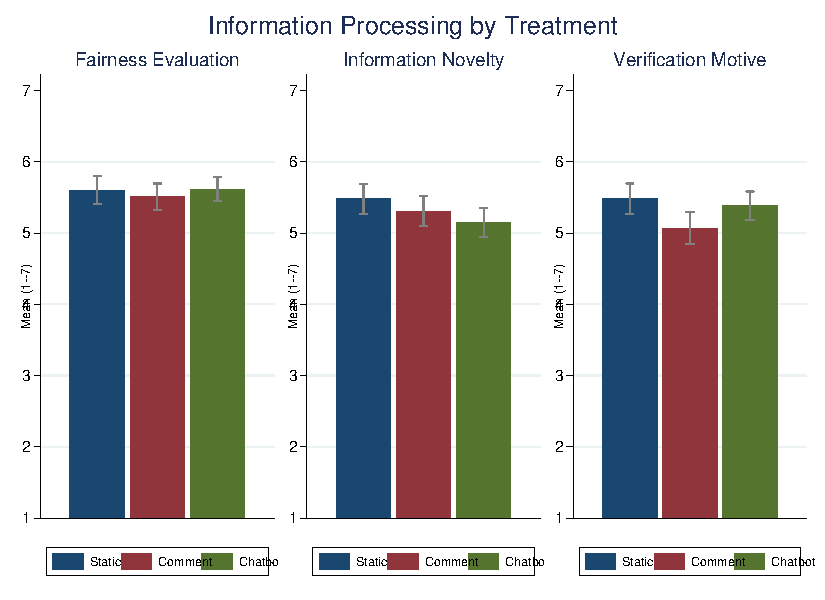
\includegraphics[width=\textwidth]{fig5_mechanisms.pdf}
\caption{Information Processing Measures by Treatment (with 95\% CIs)}
\label{fig:mech}
\end{figure}

%============================================================
\section{Summary}
%============================================================

\begin{table}[H]
\centering
\caption{Summary of Primary and Secondary Results}
\label{tab:summary_results}
\begin{tabular}{llccc}
\toprule
 & & OLS & With controls & Permutation \\
Outcome & Contrast & $\hat{\beta}$ ($p$) & $\hat{\beta}$ ($p$) & $p$ \\
\midrule
\textit{Primary} & & & & \\
\quad Bias & Chatbot vs.\ Static & 8.52 ($<$0.001) & 7.79 ($<$0.001) & $<$0.001 \\
\quad Bias & Comment vs.\ Static & 5.27 (0.008) & 5.02 (0.012) & 0.013 \\
\addlinespace
\textit{Secondary} & & & & \\
\quad One-sided & Chatbot vs.\ Static & 5.43 (0.003) & --- & 0.007 \\
\quad One-sided & Comment vs.\ Static & 5.33 (0.005) & --- & 0.008 \\
\quad Trust & Chatbot vs.\ Static & $-$1.13 (0.436) & --- & 0.445 \\
\quad Share & Chatbot vs.\ Static & 0.11 (0.931) & --- & 0.923 \\
\bottomrule
\end{tabular}
\par\vspace{4pt}
\begin{minipage}{\textwidth}
\footnotesize \textit{Notes:} OLS estimates from regressions controlling for pre-treatment outcome level. ``With controls'' adds demographics and country fixed effects. Static is the omitted baseline. Primary contrasts survive Bonferroni-Holm (pairwise) and Romano-Wolf (outcome family) corrections.
\end{minipage}
\end{table}

The central finding is that both AI-based interventions---the interactive chatbot and the tailored comment---significantly increase perceived bias against China relative to a static message. With the expanded three-country sample ($N=1{,}017$), the Comment effect, which was insignificant in the two-country sample, now reaches significance ($p=0.008$; Westfall-Young adjusted $p=0.015$). Both interventions also increase perceived one-sidedness, but neither differentially affects trustworthiness or sharing intentions. Treatment effects are consistent across the US, UK, and Canada.

We emphasize two important limitations. First, the experiment identifies shifts in \textit{perceived} bias, not whether the induced perceptions are accurate or welfare-improving. Second, the design cannot separate the effect of interactivity from the effect of message content: the chatbot was designed to highlight potential anti-China bias in the article, so the estimated effect reflects exposure to that framing.

\end{document}
